\begin{frame}
\frametitle{From generic to ringmap}
\begin{columns}
\column[t]{0.5\textwidth}
\vspace{-1em}
\begin{itemize}
	\item<1->\textbf{generic}
	\item<2->Eliminate packet copies  and syscalls
	\item<3->BPF-Buffer is then not necessary
		\begin{itemize}
			\item<3->Packet filtering is possible in both kernel and 
				user-space
		\end{itemize}
	\item<4->Mapping the Packet-Buffer to user-space
	\item<5->[$\Rightarrow$]\textbf{ringmap}
\end{itemize}
\column[t]{0.5\textwidth}
\vspace{-2em}
\only<1>{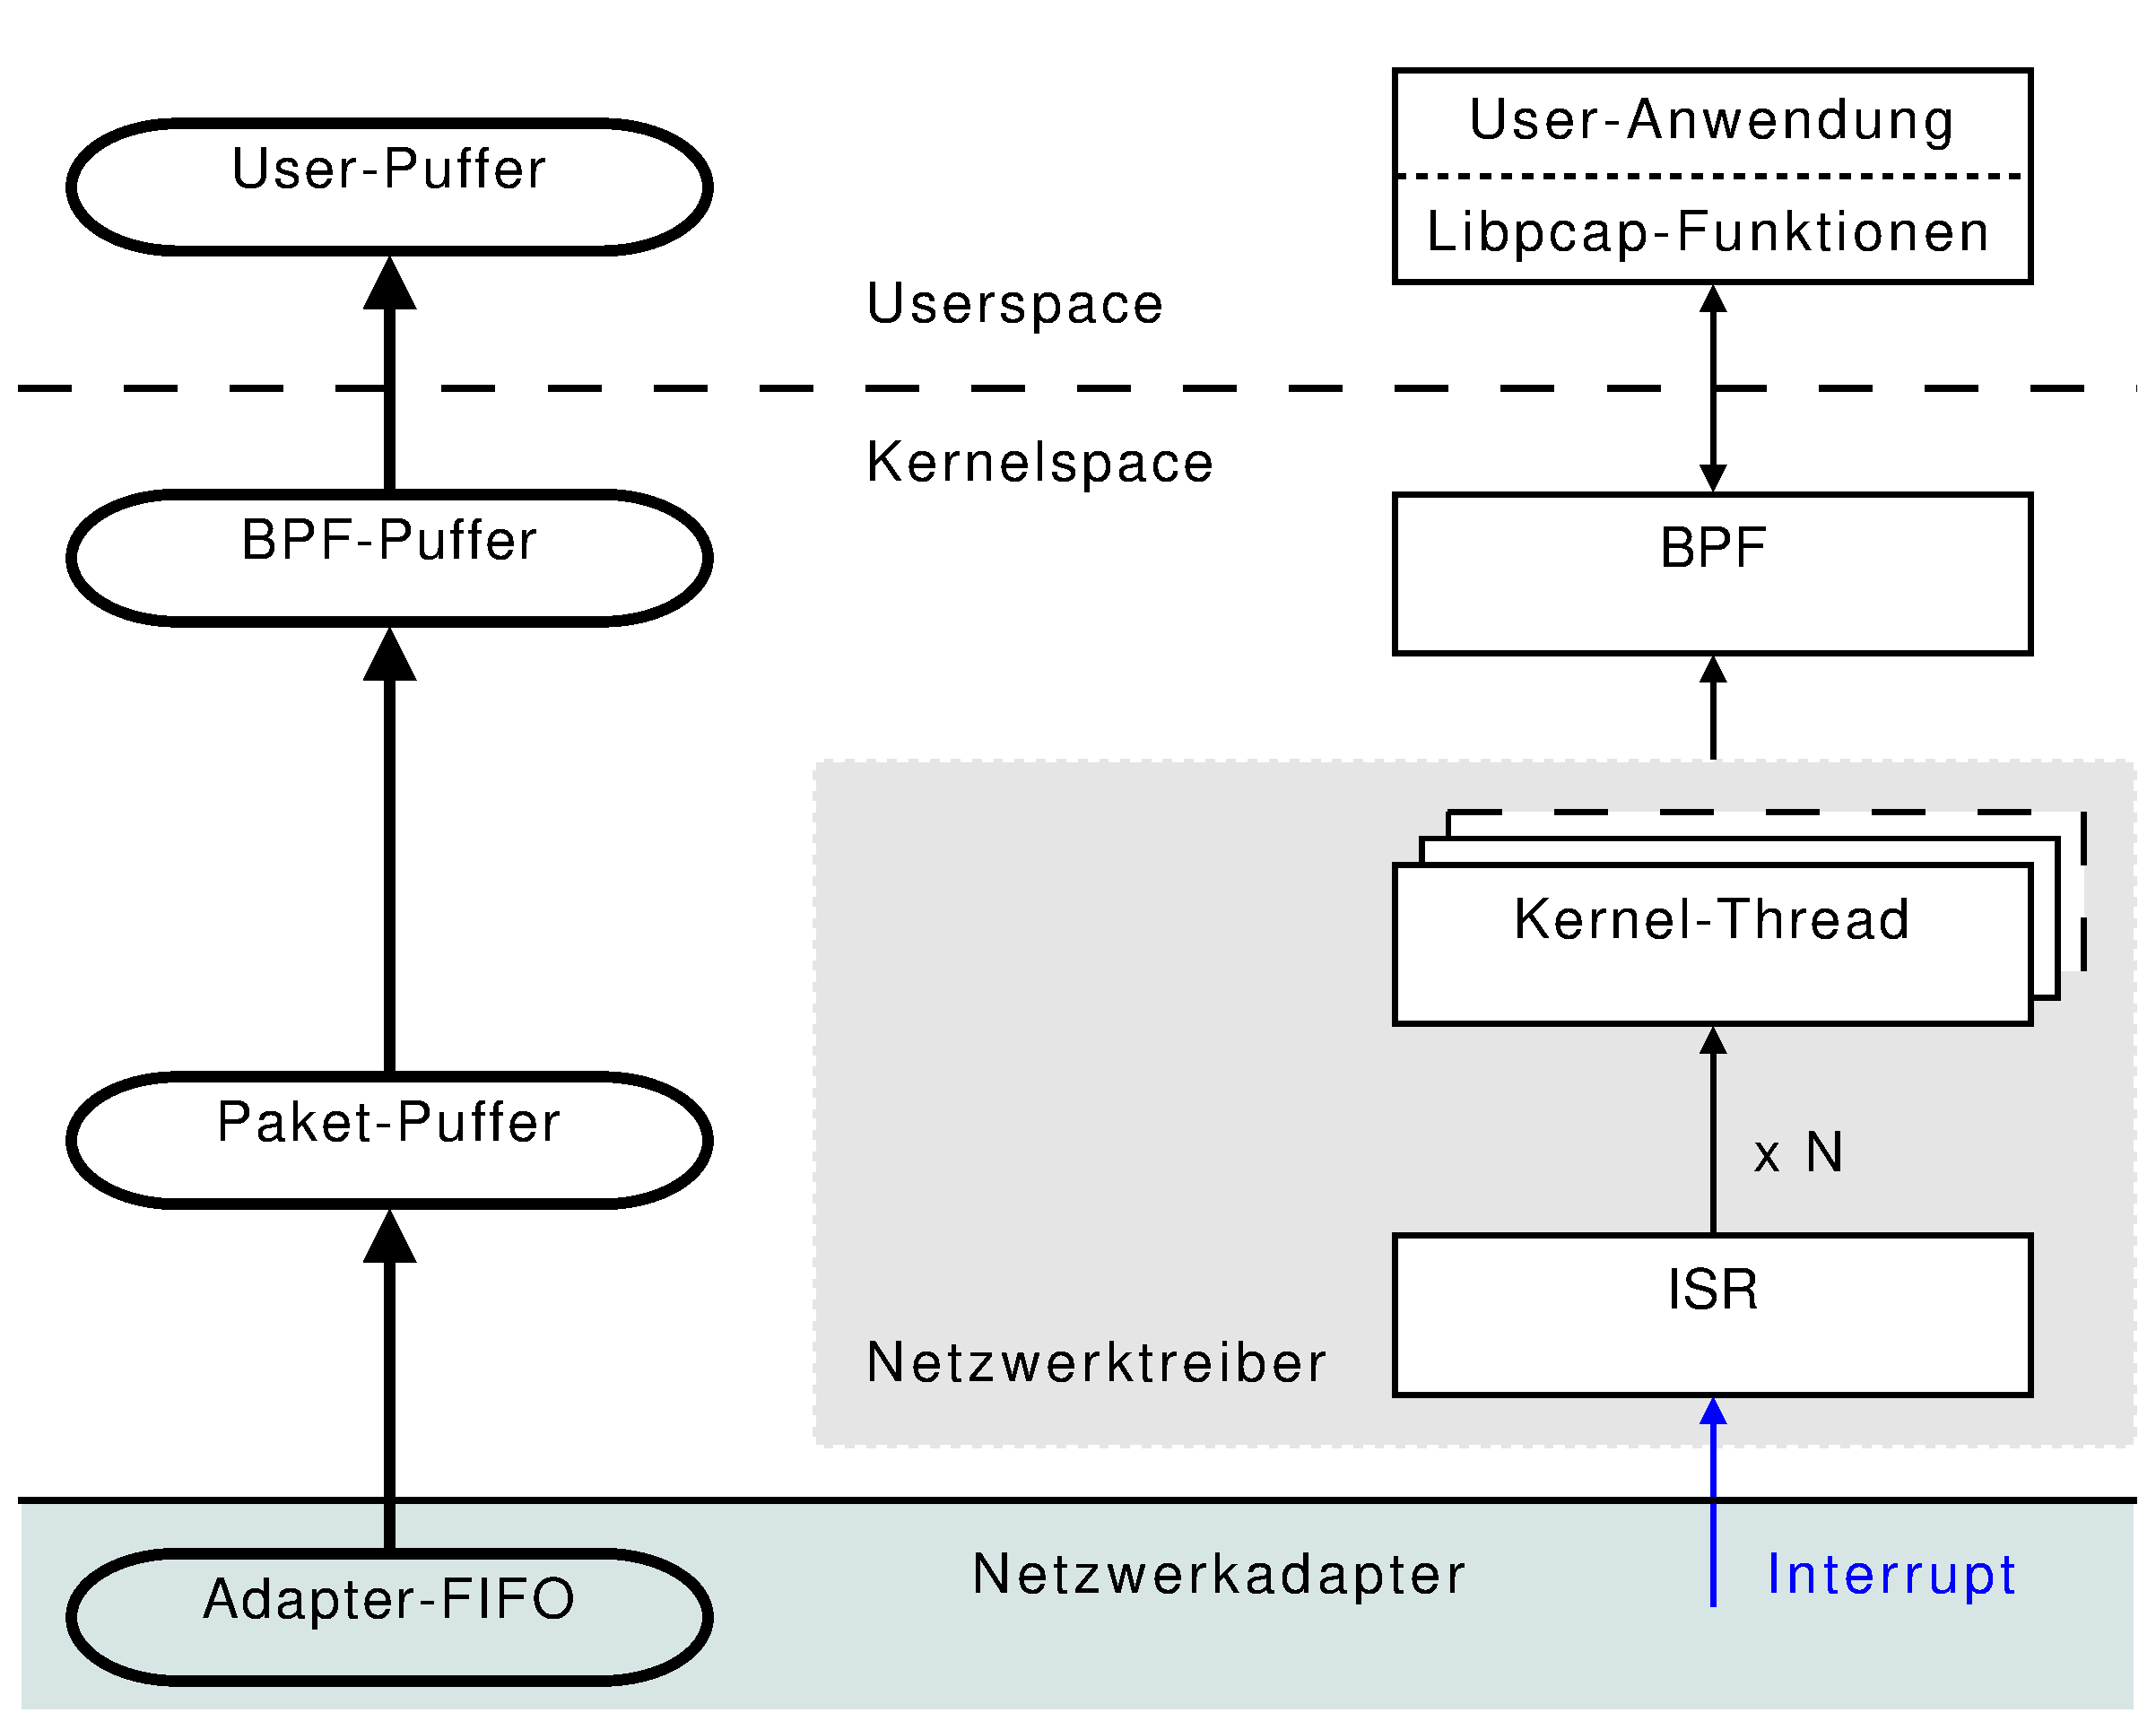
\includegraphics [height=59mm,width=60mm]{pics/3copy}}
\only<2>{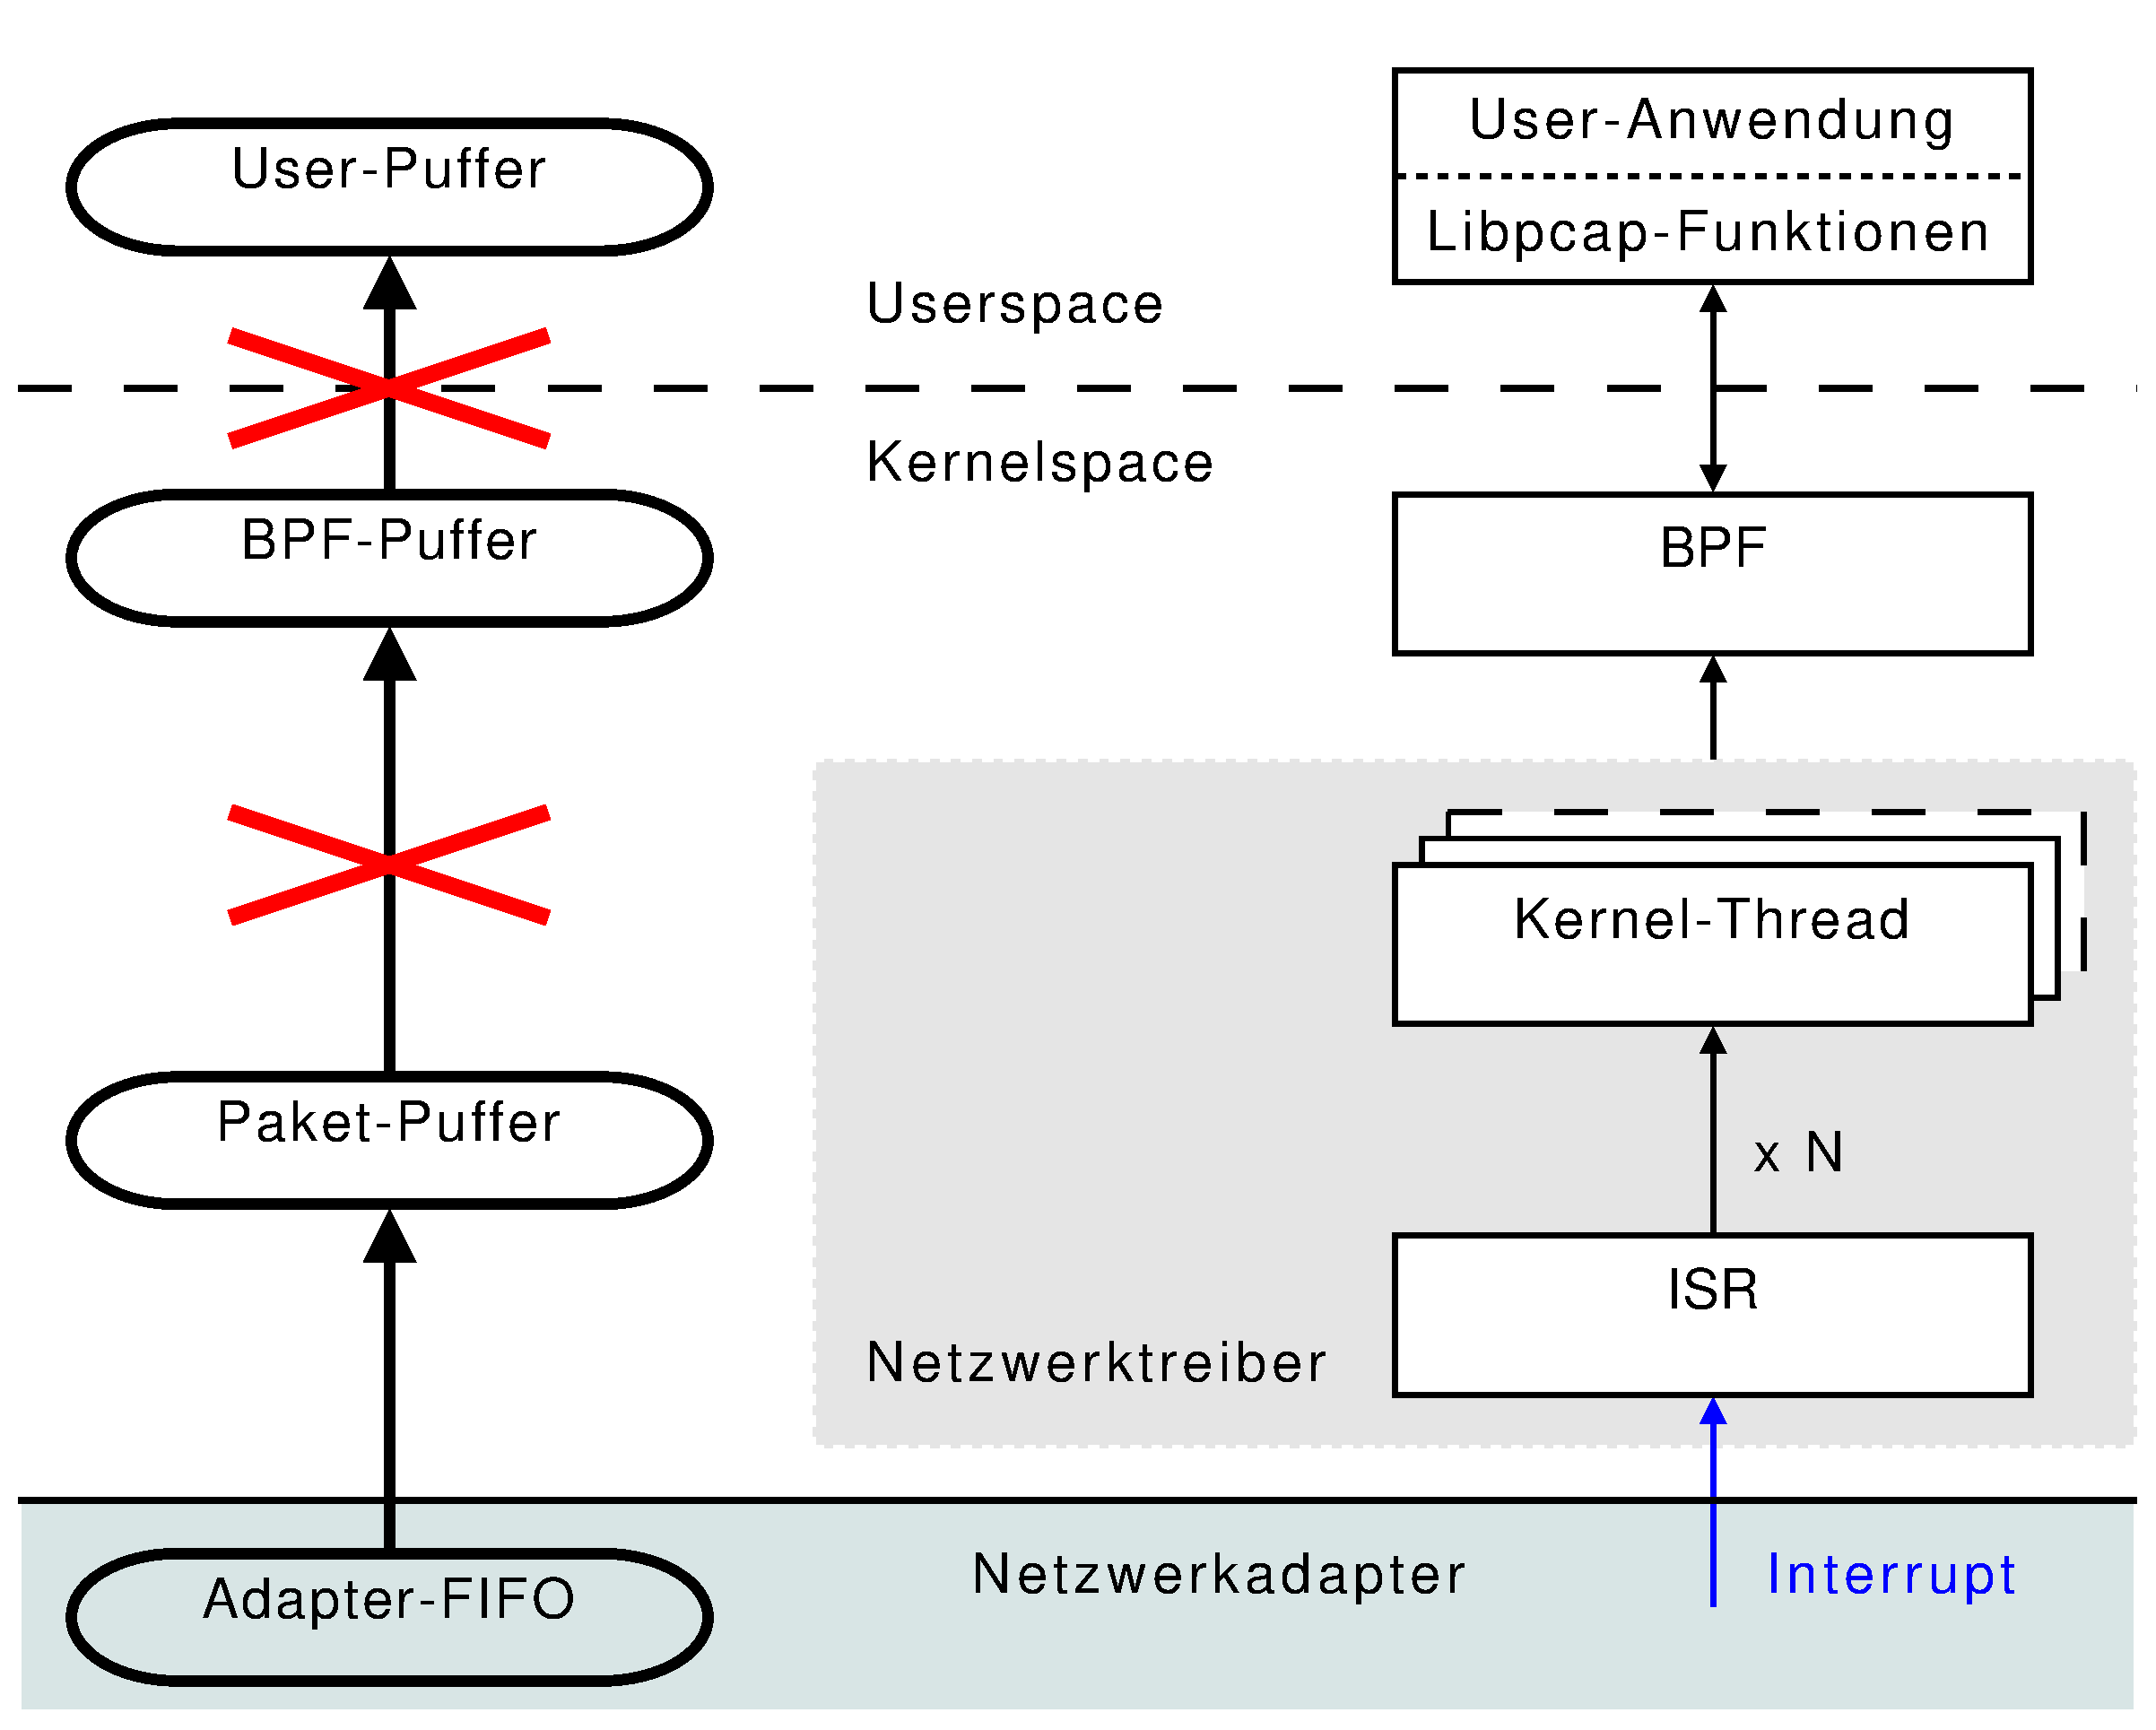
\includegraphics [height=59mm,width=60mm]{pics/3copy_solution_1}}
\only<3>{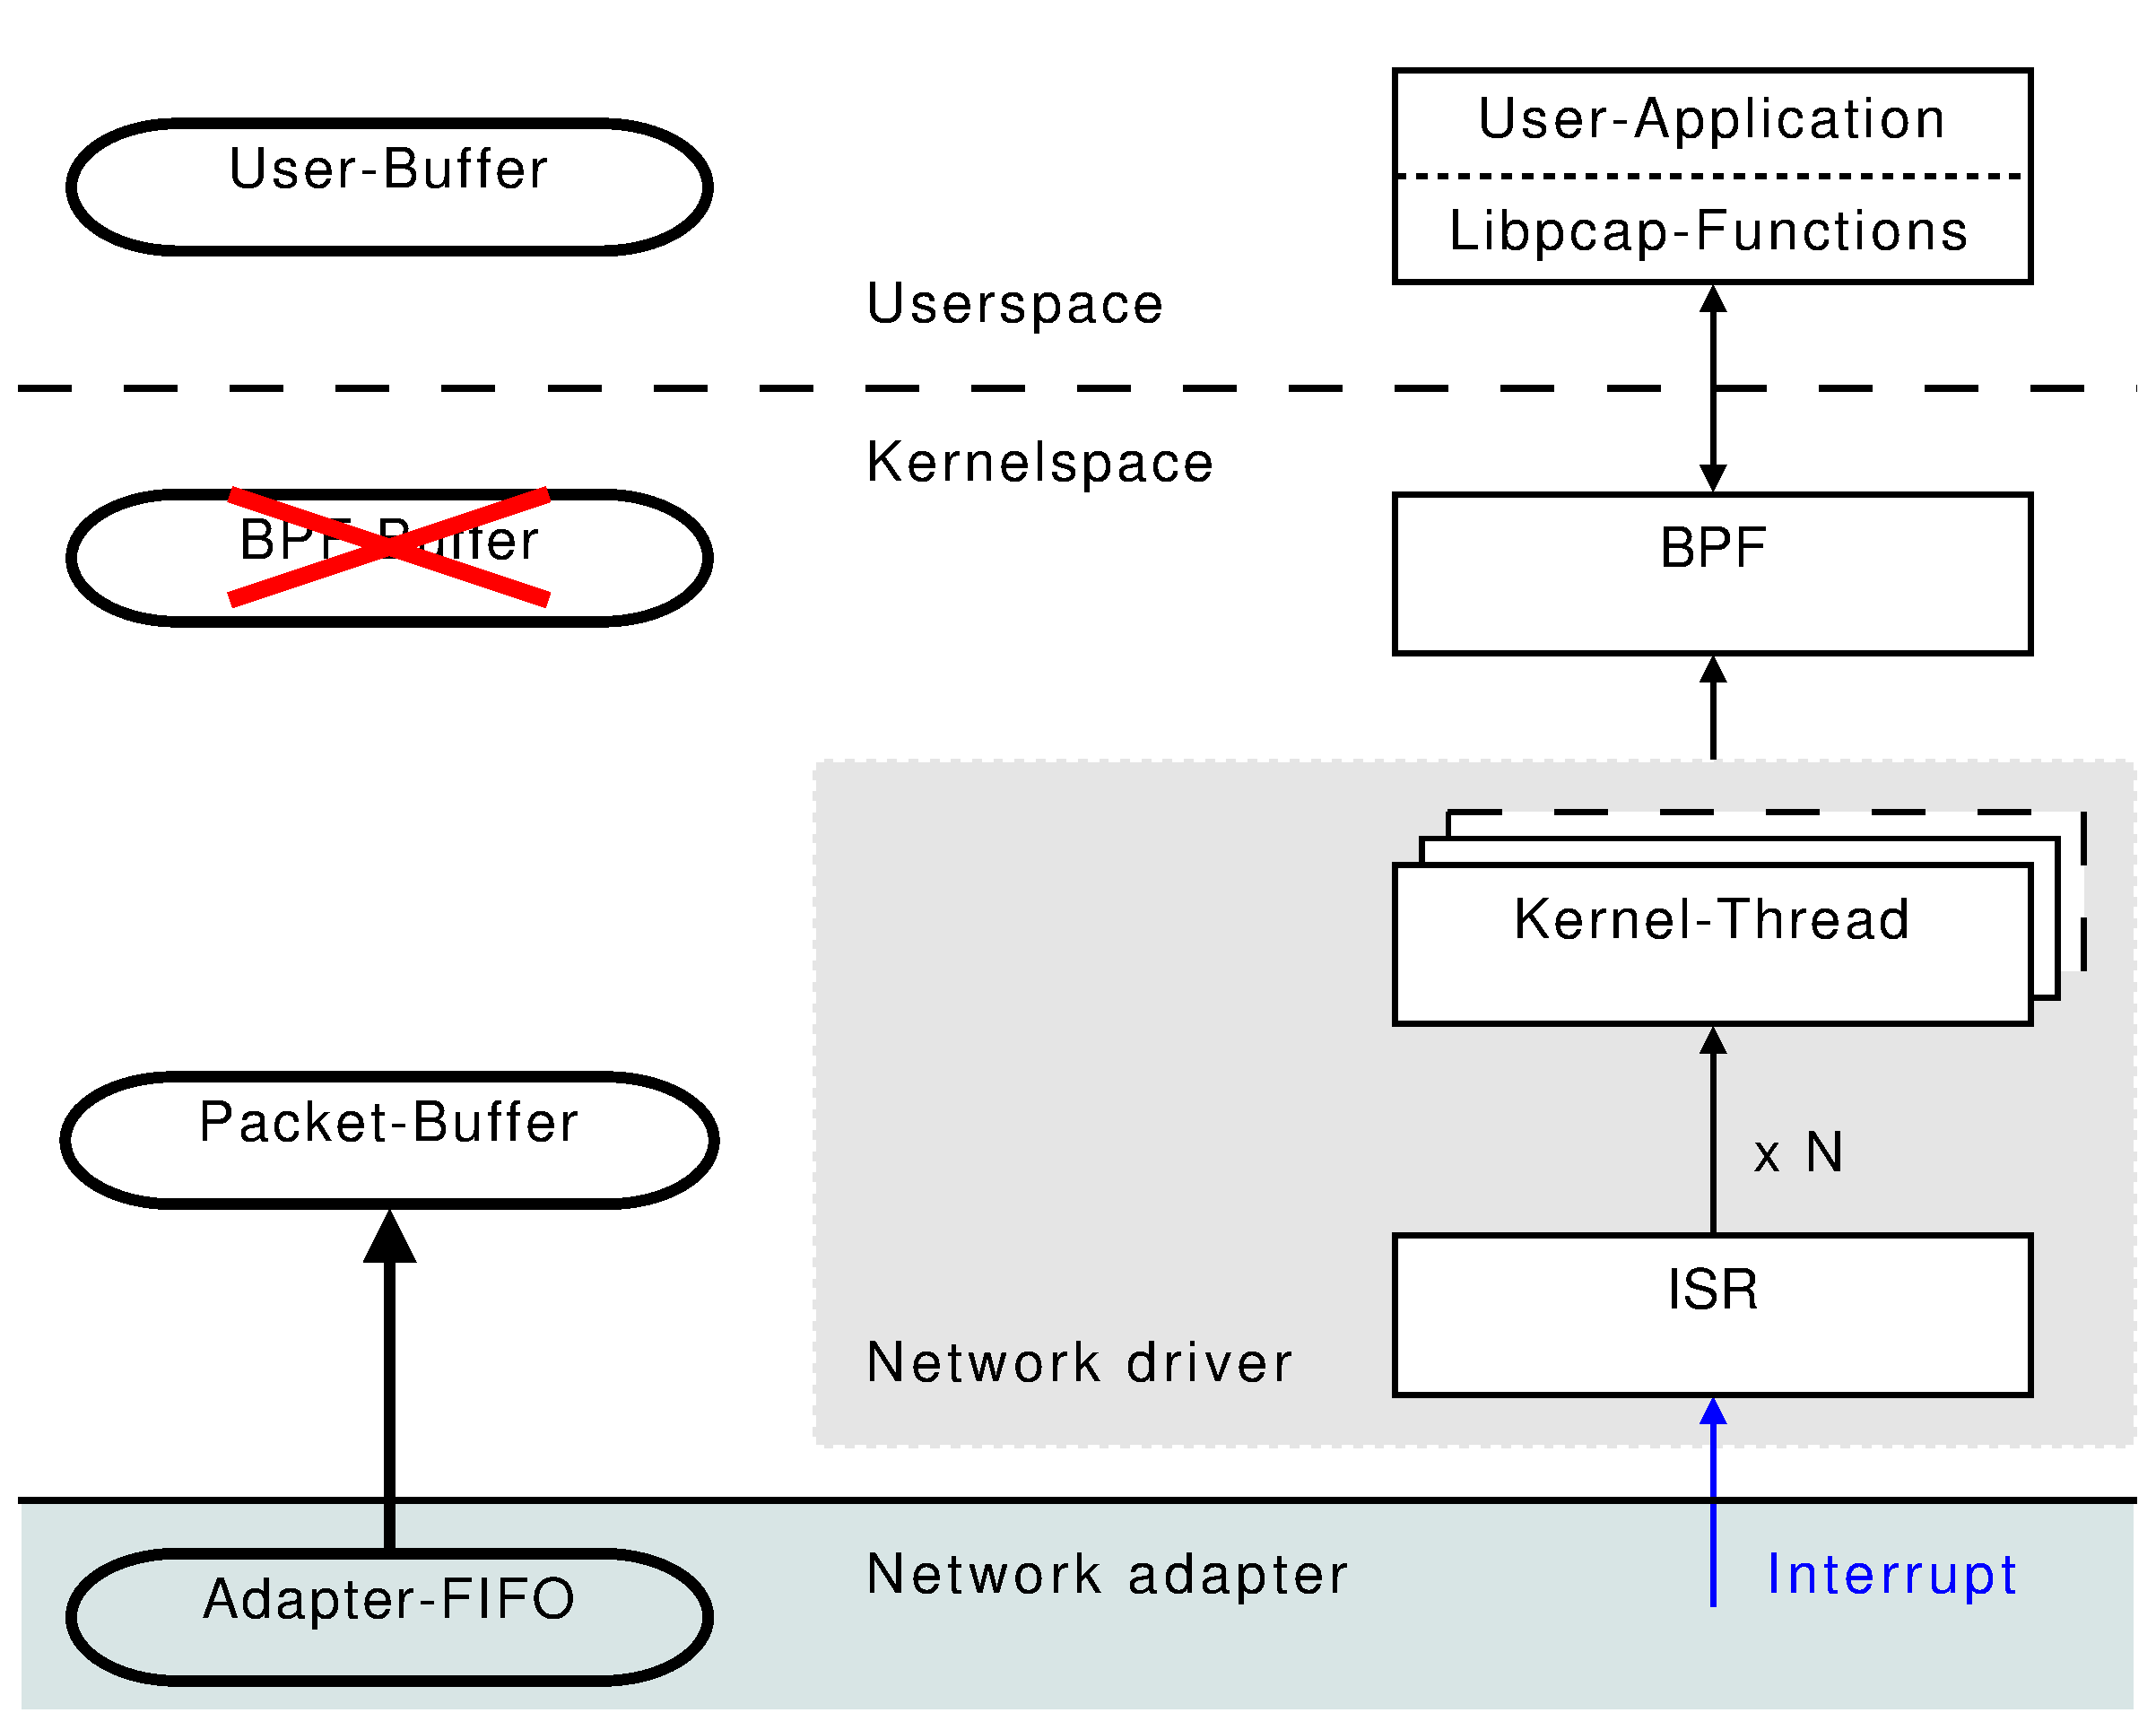
\includegraphics [height=59mm,width=60mm]{pics/3copy_solution_2}}
\only<4>{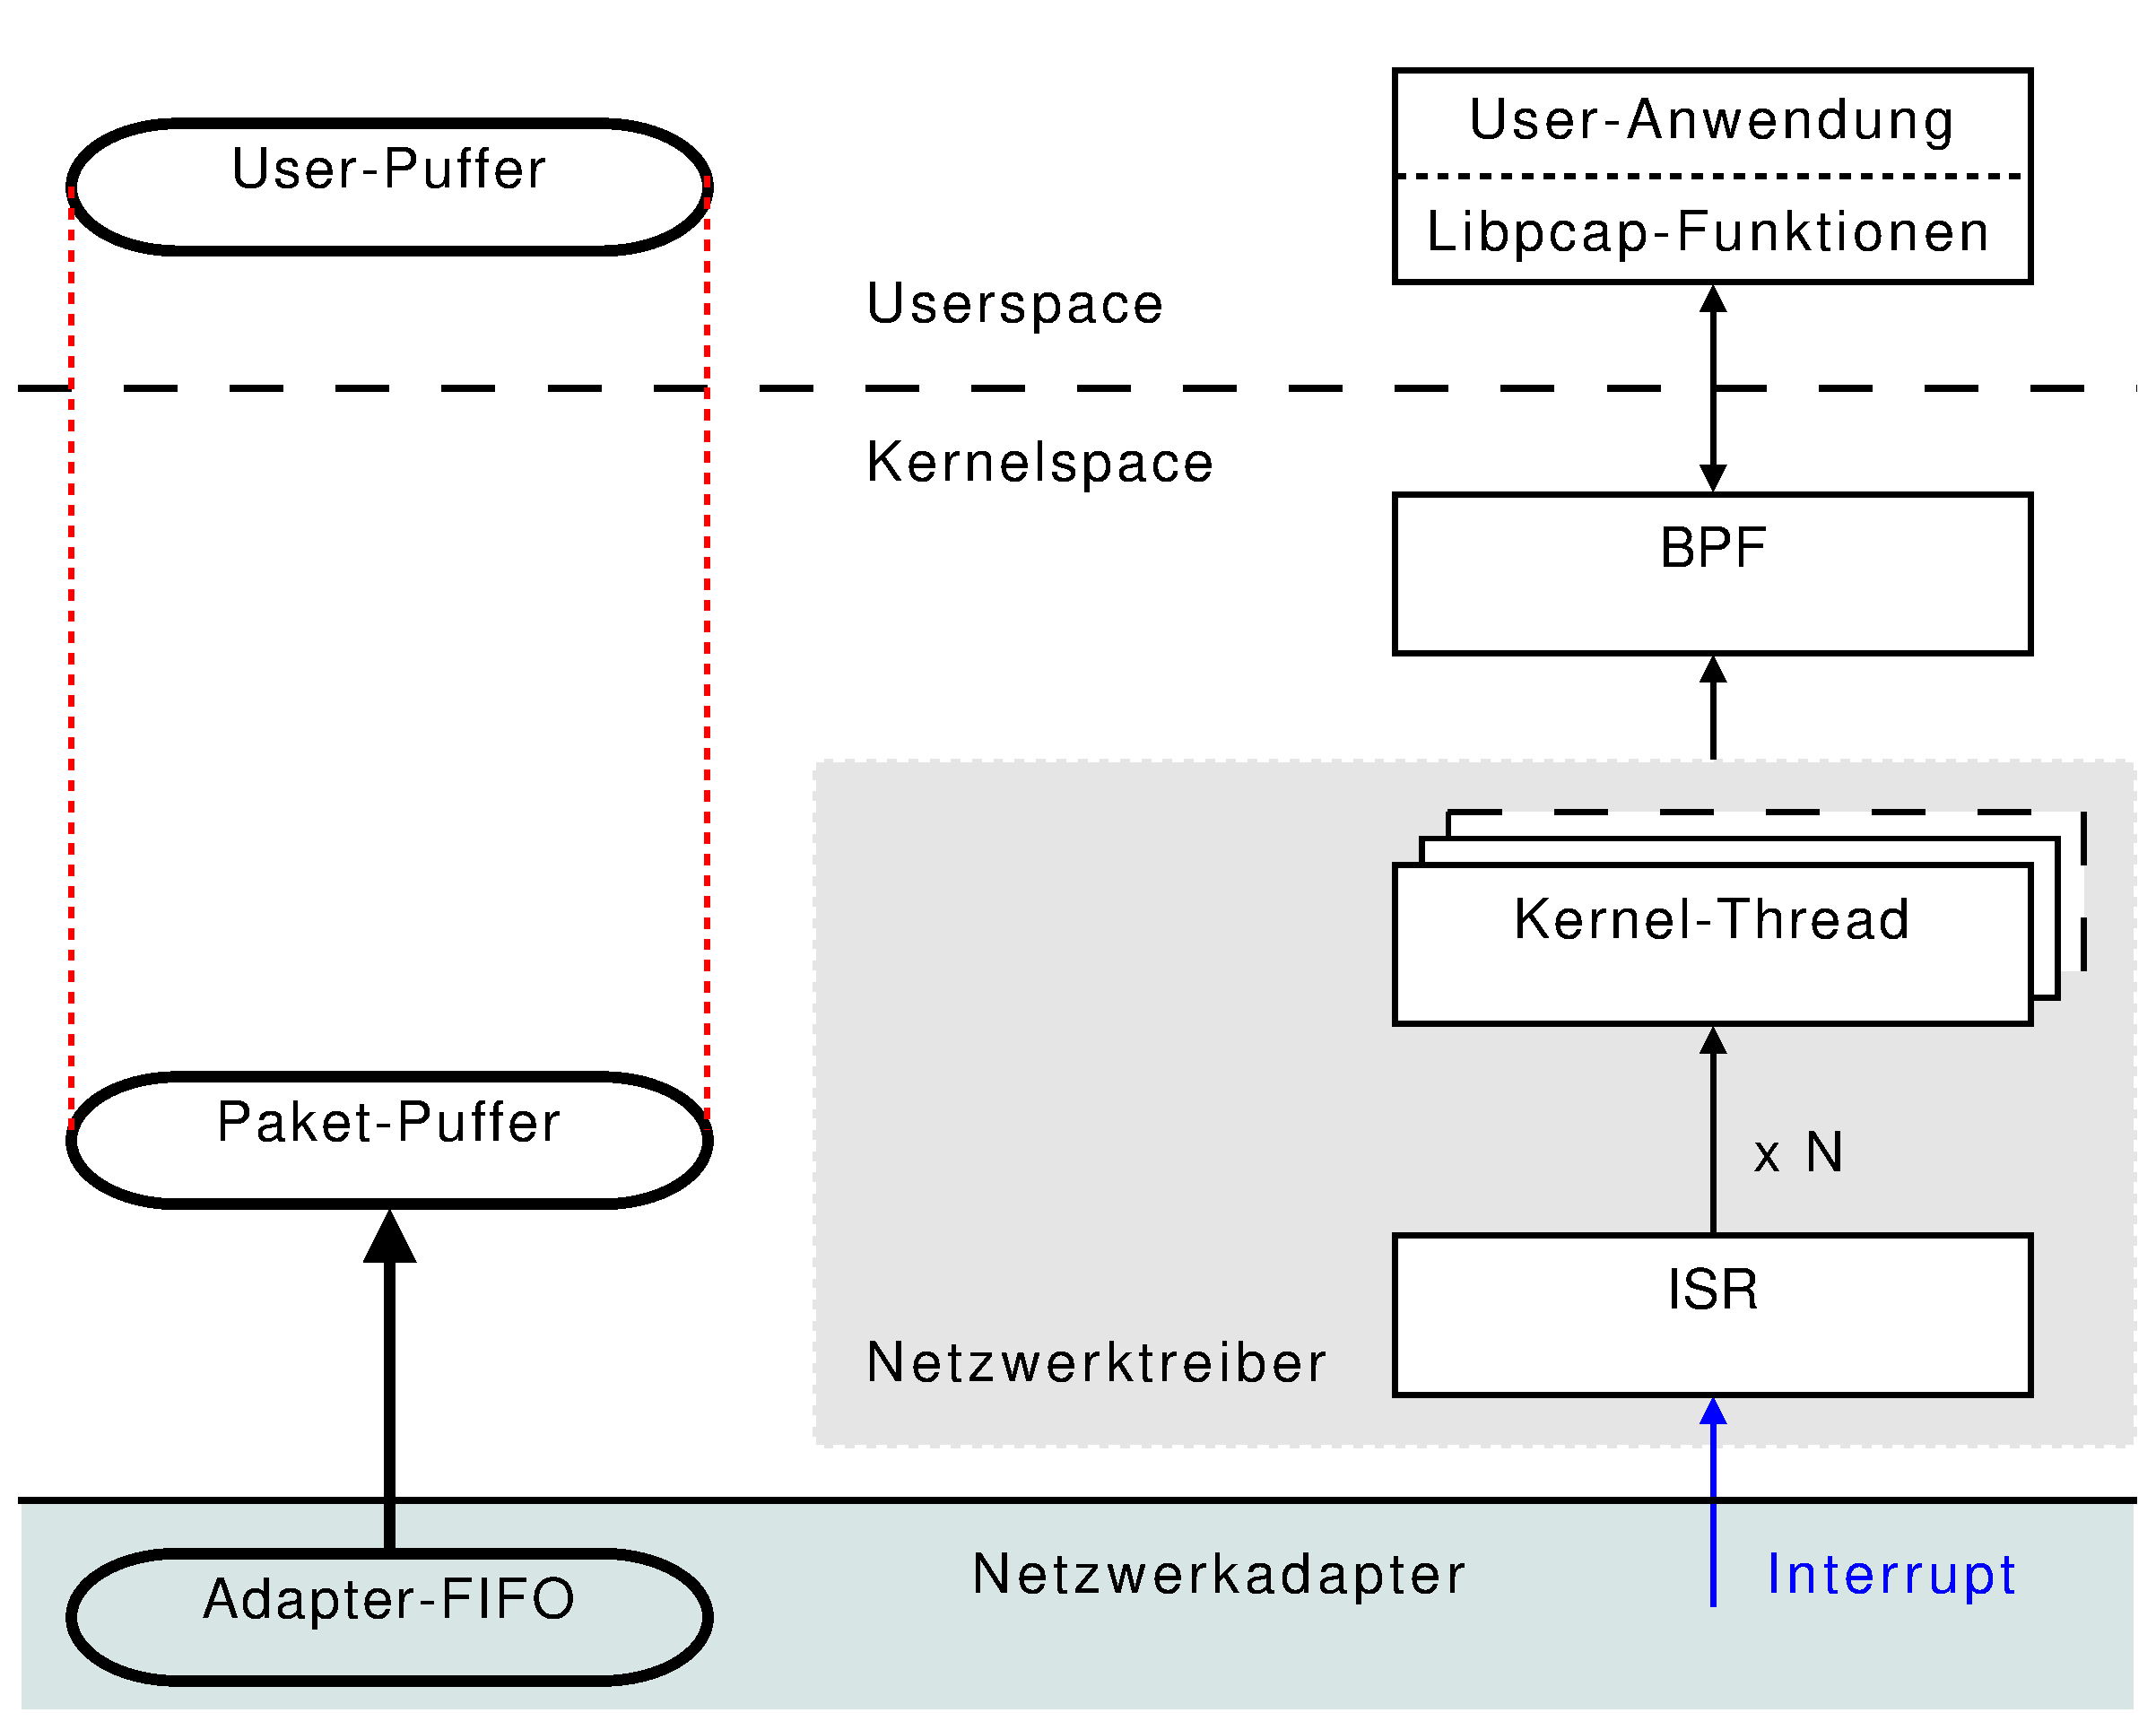
\includegraphics [height=59mm,width=60mm]{pics/3copy_solution_3}}
%\only<5>{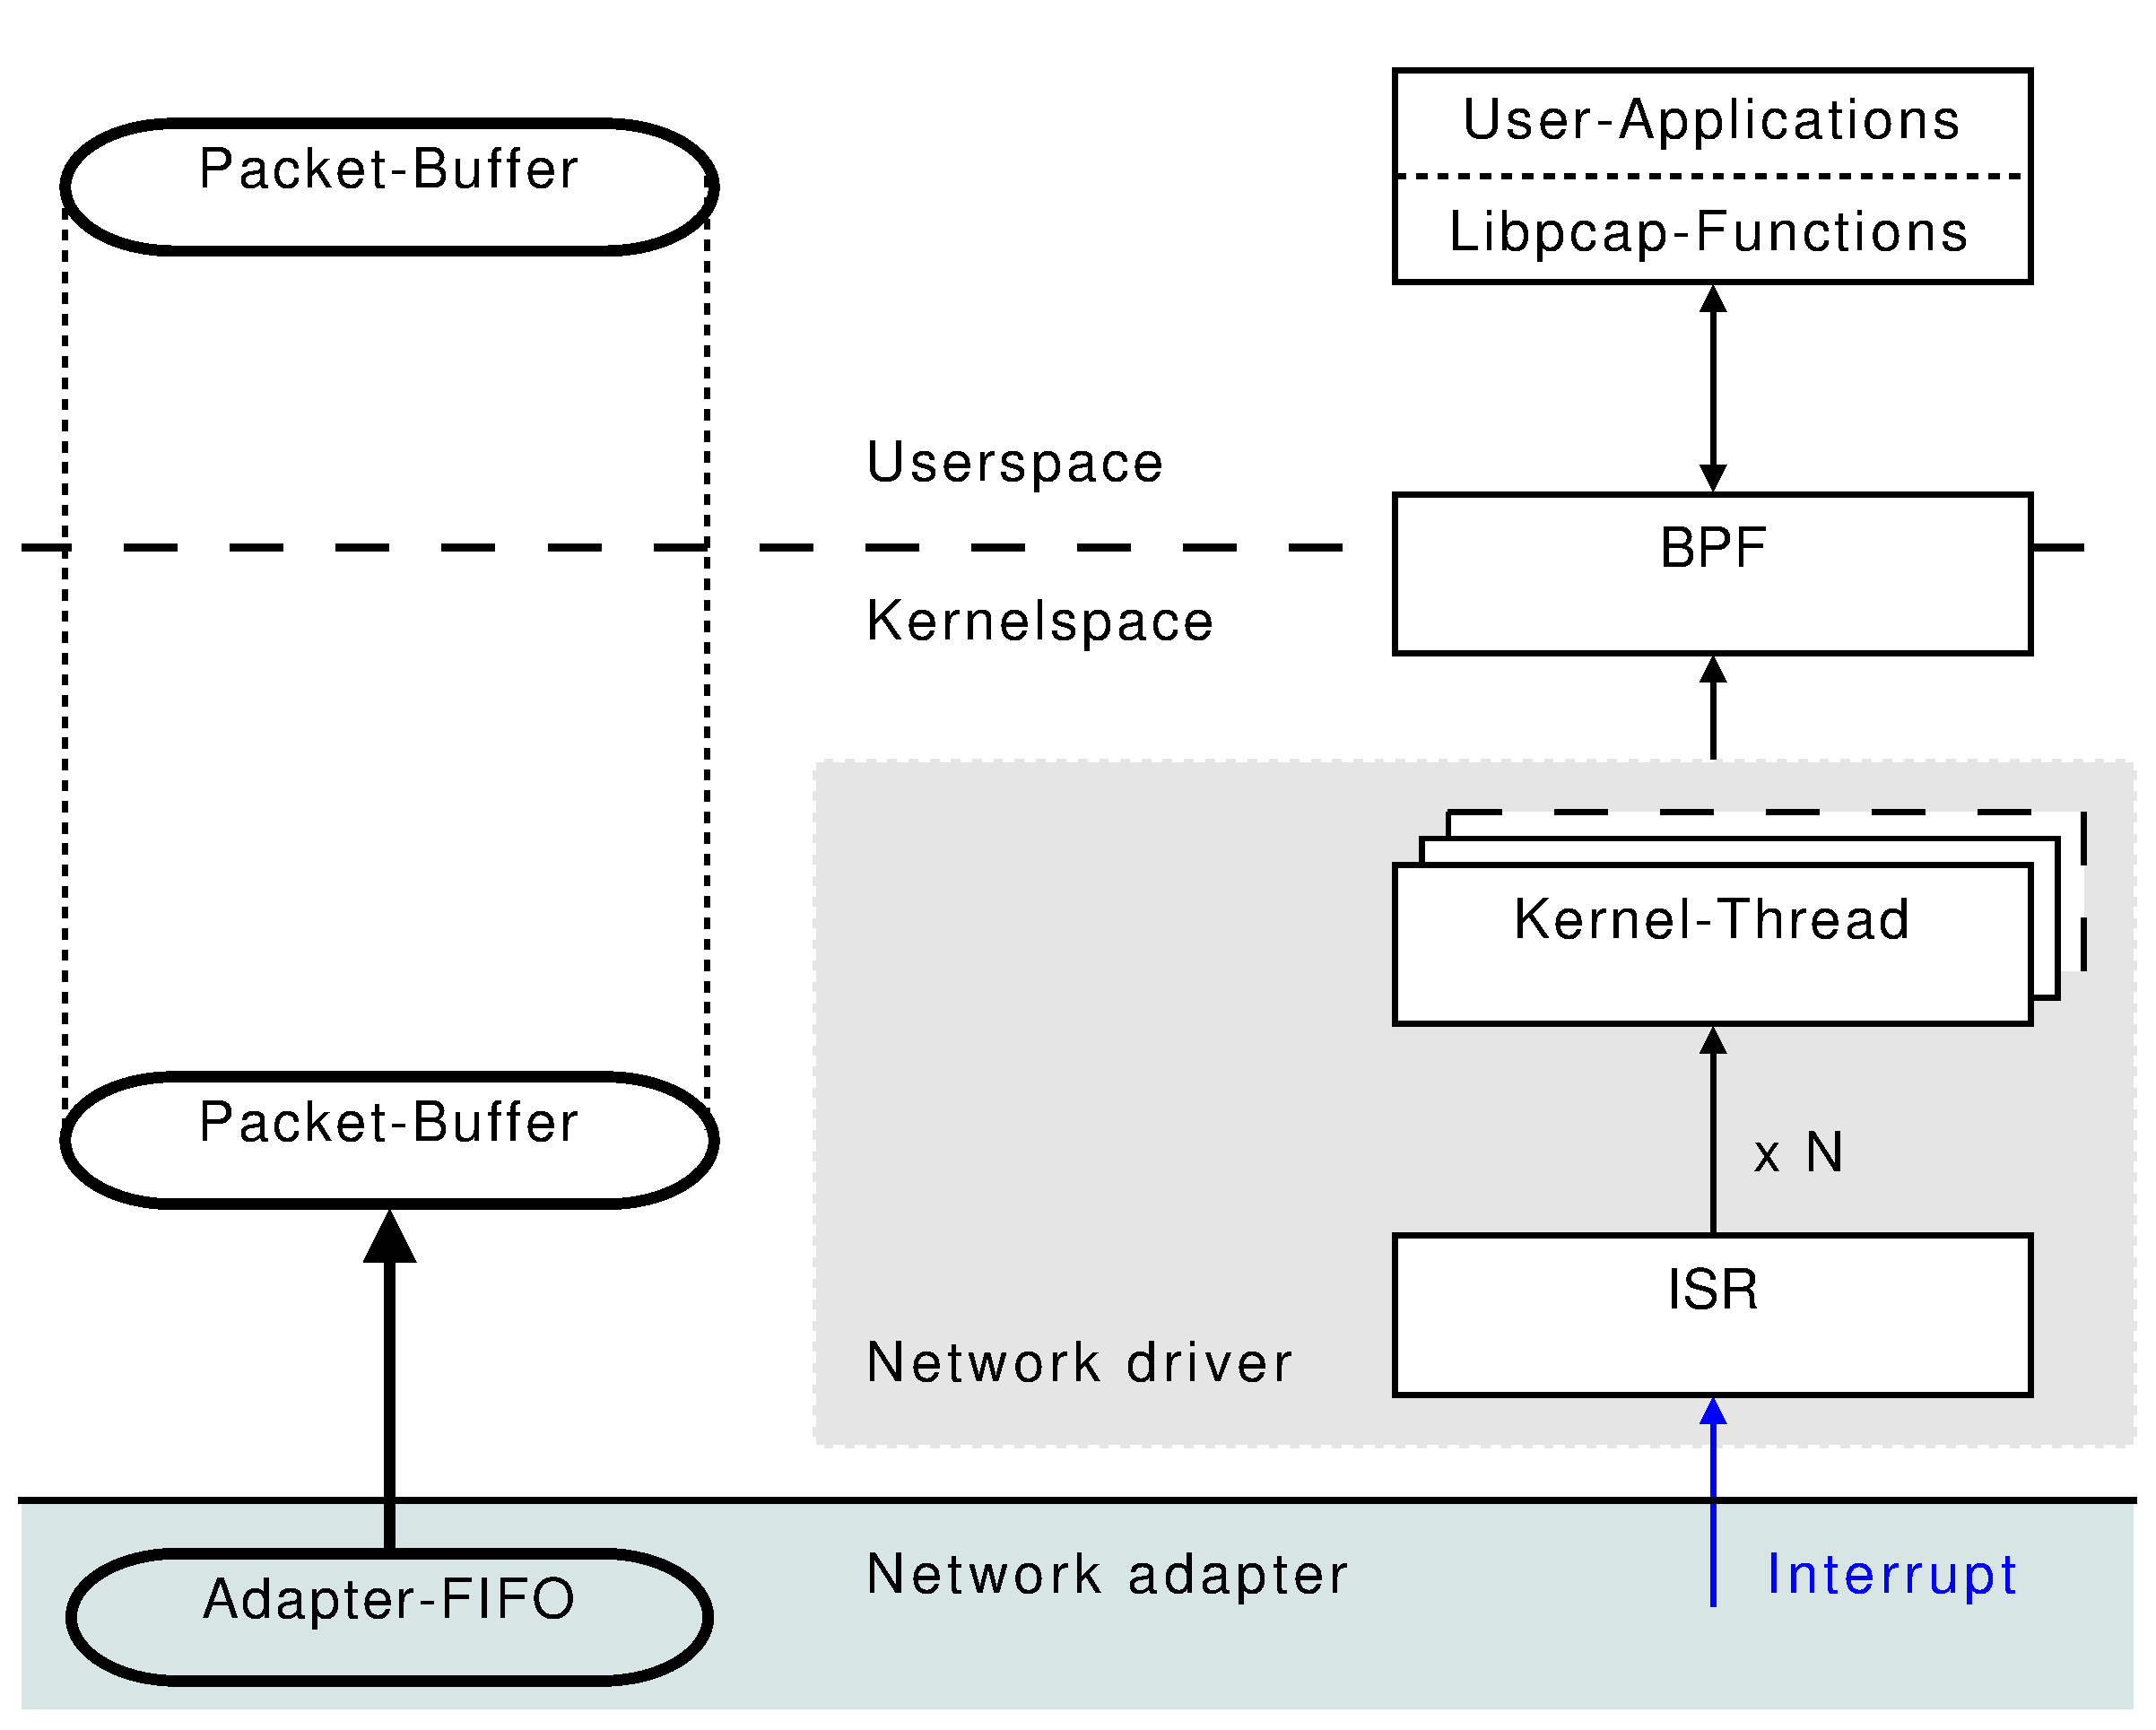
\includegraphics [height=59mm,width=60mm]{pics/3copy_solution_4}}
\only<5>{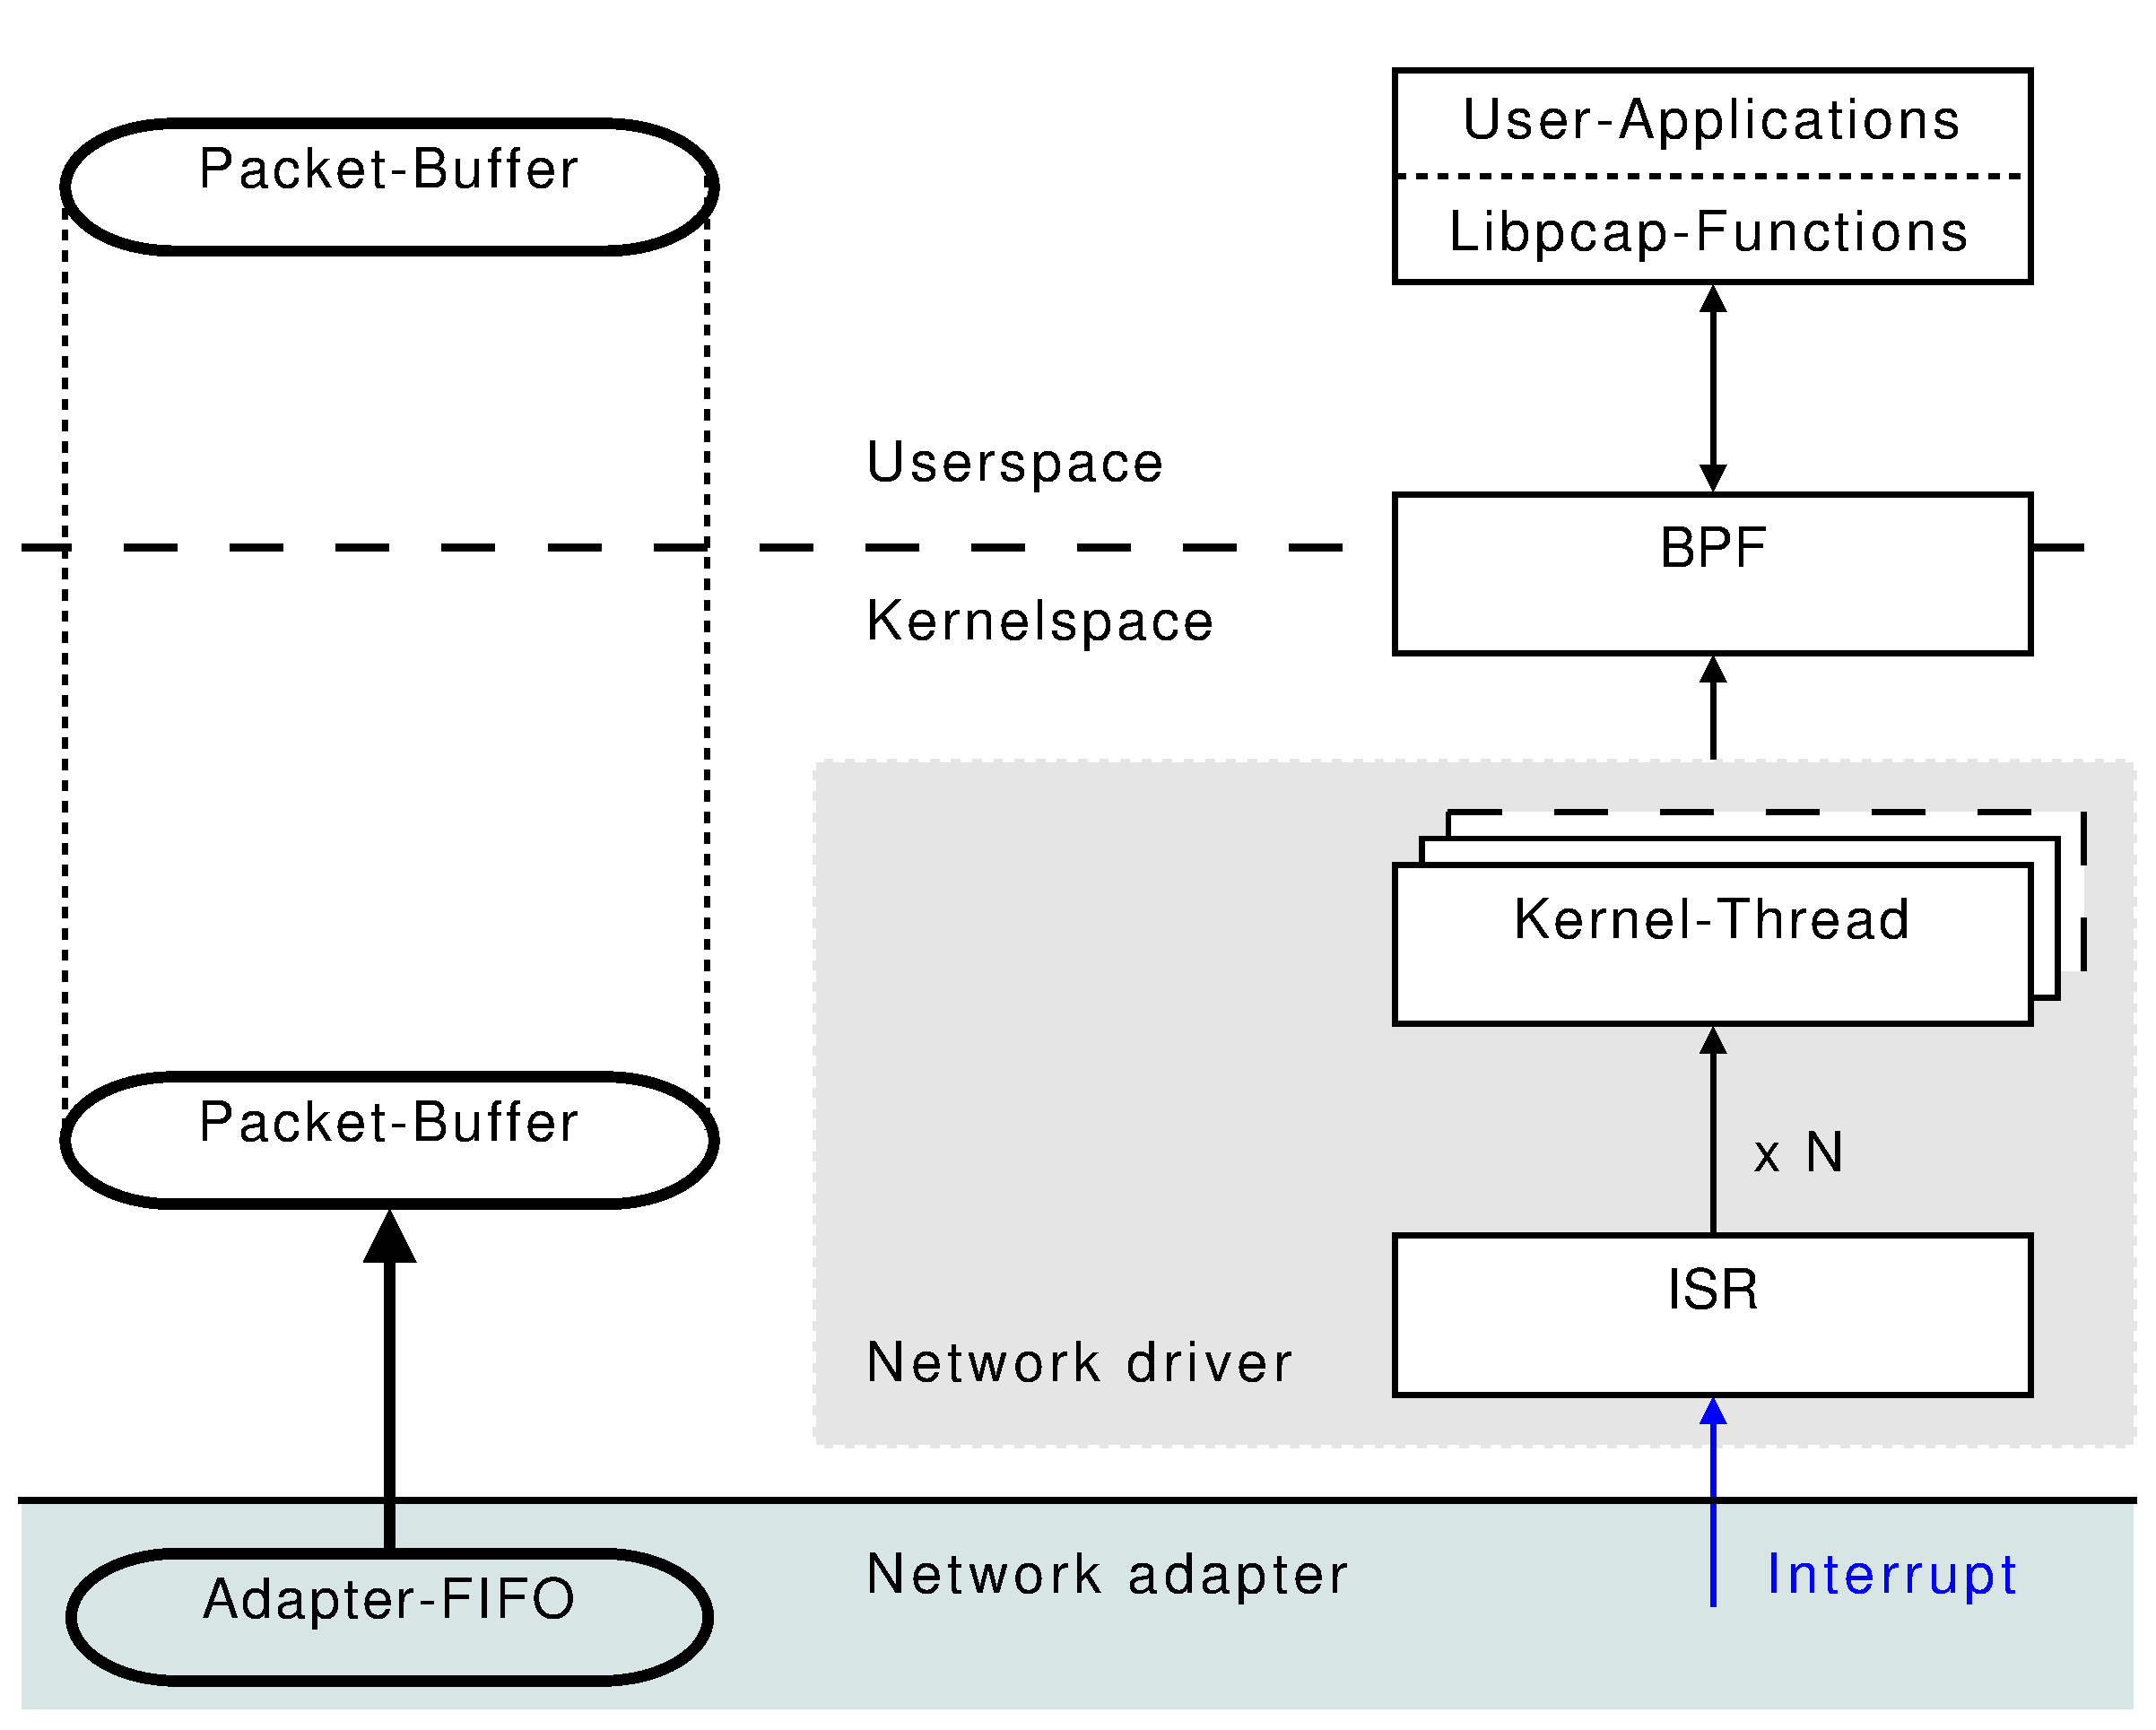
\includegraphics [height=59mm,width=60mm]{pics/3copy_solution_4}}
\end{columns}
\end{frame}

